% 0095(본책 21쪽) — ∠C=90° 직각삼각형 ABC(B 왼쪽 아래·C 오른쪽 아래·A 위로 길게), AC 위의 D(AD=BD), ∠DBC=60°, BC=5 파선 호. 라벨: A~D·60°·5, 같은 길이 표시(AD=BD), 직각 표시 C. 스캔 삽화를 TikZ 로 다시 그림. 답(tan 75°)은 적지 않는다.
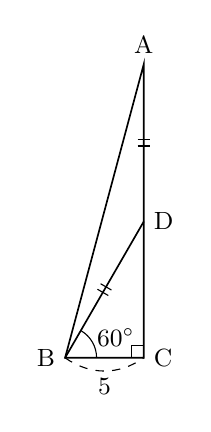
\begin{tikzpicture}[scale=1, line width=0.6pt]
  \coordinate (B) at (0,0); \coordinate (C) at (1.0,0); \coordinate (D) at (1.0,1.732); \coordinate (A) at (1.0,3.732);
  \draw (A) -- (B) -- (C) -- cycle;
  \draw (B) -- (D);
  % 직각 표시(C)
  \draw[line width=0.4pt] (0.84,0) -- (0.84,0.16) -- (1.0,0.16);
  % 60°
  \draw[line width=0.4pt] (0.4,0) arc[start angle=0, end angle=60, radius=0.4cm];
  \node[font=\small, anchor=west, inner sep=1pt] at (0.36,0.26) {$60^\circ$};
  % 같은 길이 표시(AD=BD)
  \draw[line width=0.4pt] (0.92,2.69) -- (1.08,2.69) (0.92,2.77) -- (1.08,2.77);
  \draw[line width=0.4pt] (0.411,0.871) -- (0.549,0.791) (0.451,0.941) -- (0.589,0.861);
  % 5(BC 파선 호)
  \draw[dashed, line width=0.4pt] (B) to[bend right=35] (C);
  \node[font=\small] at (0.5,-0.36) {$5$};
  \node[font=\small, above] at (A) {A};
  \node[font=\small, left] at (B) {B};
  \node[font=\small, right] at (C) {C};
  \node[font=\small, right] at (D) {D};
\end{tikzpicture}
